\documentclass[times,twocolumn,final,authoryear]{elsarticle}

%% Stylefile to load PR Letters template
\usepackage{prletters}
\usepackage{framed,multirow}

%% The amssymb package provides various useful mathematical symbols
\usepackage{amssymb}
\usepackage{latexsym}

% Following three lines are needed for this document.
% If you are not loading colors or url, then these are
% not required.
\usepackage{url}
\usepackage{xcolor}
\definecolor{newcolor}{rgb}{.8,.349,.1}

%%%%% previous paper packages
\usepackage[ruled]{algorithm2e}
\usepackage{subfig}
%%%%%

\journal{Pattern Recognition Letters}

\begin{document}

\thispagestyle{empty}
 

\begin{table*}[!th]
\ifpreprint\else\vspace*{-5pc}\fi

\section*{Research Highlights (Required)}

%To create your highlights, please type the highlights against each
%\verb+\item+ command. 

\vskip1pc

\fboxsep=6pt
\fbox{
\begin{minipage}{.95\textwidth}
%It should be short collection of bullet points that convey the core
%findings of the article. It should  include 3 to 5 bullet points
%(maximum 85 characters, including spaces, per bullet point.)  
\vskip1pc
\begin{itemize}

 \item Definition of sufficient sanitizer to protect privacy with utility guarantees.

 \item SwapMob algorithm is a sufficient sanitizer for real-time mobility data collection.

 \item Application to obtain Origin-Destination matrices that preserve privacy. 
 
 
\end{itemize}
\vskip1pc
\end{minipage}
}

\end{table*}

\clearpage


\ifpreprint
  \setcounter{page}{1}
\else
  \setcounter{page}{1}
\fi
%UNCOMMENT previous

\begin{frontmatter}

\title{Swapping trajectories with a sufficient sanitizer}

%%%%%%%%%%

\author[1,2]{Juli\'an \snm{Salas}\corref{cor1}} 
\cortext[cor1]{Corresponding author: 
  Tel.: +34-933-263-651}
\ead{jsalaspi@uoc.edu}

\author[1,2]{David \snm{Meg\'ias}}
\author[3,4]{Vicen\c{c}  \snm{Torra}}
\author[5]{Marina  \snm{Toger}}
\author[6]{Joel  \snm{Dahne}}
\author[6,7]{Raazesh  \snm{Sainudiin}}

\address[1]{Internet Interdisciplinary Institute (IN3), Universitat Oberta de Catalunya (UOC), Barcelona, Spain.
}
\address[2]{CYBERCAT-Center for Cybersecurity Research 
of Catalonia, Barcelona, Spain.}
\address[3]{Hamilton Institute, Maynooth University, Maynooth, Ireland.}
\address[4]{School of Informatics, University of Sk\"{o}vde, Sk\"{o}vde, Sweden.}
\address[5]{Department of Economic and Cultural Geography, Uppsala University, Uppsala, Sweden.}
\address[6]{Department of Mathematics, Uppsala University, Uppsala, Sweden.}
\address[7]{Combient Competence Centre for Data Engineering Sciences, Uppsala University, Sweden.}

\begin{abstract}

Real-time mobility data is useful for several applications such as planning transports in metropolitan areas or localizing services in towns. However, if such data is collected without any privacy protection it may reveal sensible locations and pose safety risks to an individual associated to it.
Thus, mobility data must be anonymized preferably at the time of collection.

In this paper, we consider the SwapMob algorithm that mitigates privacy risks by swapping partial trajectories. We formalize the concept of sufficient sanitizer and show that the SwapMob algorithm is a sufficient sanitizer for various statistical decision problems. That is, it preserves the aggregate information of the spatial database in the form of sufficient statistics and also provides privacy to the individuals. 
This may be used for personalized assistants taking advantage of users' locations, so they can ensure user privacy while providing accurate response to the user requirements.

We measure the privacy provided by SwapMob as the Adversary Information Gain, which measures the capability of an adversary to leverage his knowledge of exact data points to infer a larger segment of the sanitized trajectory. 
We test the utility of the data obtained after applying SwapMob sanitization in terms of Origin-Destination matrices, a fundamental tool in  transportation modelling.


\end{abstract}




\begin{keyword}
%\MSC *** %41A05\sep 41A10\sep 65D05\sep 65D17
\KWD Privacy Preserving Mobility Data Mining \sep Real-time mobility data anonymization \sep Trajectory anonymization \sep Sufficient Sanitizer \sep Intelligent Transportation Systems \sep Origin-Destination matrices 
\end{keyword}

\end{frontmatter}


\section{Introduction}

An increasing amount of location data is obtained from GPS, GSM and RFID technologies that may be integrated to our personal devices, such as our smartphones. This yields the opportunity of developing Location Based Services (LBS) that deliver content depending on users' locations.

However, revealing users' locations may have some privacy risks. If the data is linked to their real identities it may reveal personal preferences (e.g., sexual, political or religious orientation), or it may be used for inferring habits and knowing the time when a person is at home or away.
To avoid such inconveniences, a variety of anonymization techniques have been developed to hide the identity of the user or her exact location, cf. \cite{Terrovitis:2011}.

We can consider privacy of location data when data is protected after it has been collected, or when when users make location based queries, in this case privacy should be provided for location-based services (LBS), so that the users' privacy is protected from service providers. 

A well established approach for privacy protection in LBS is using Mix Zones, cf. \cite{Beresford2003}.
Mix zones are regions in which applications cannot trace user movements. 
Inside a mix zone, applications receive users pseudonyms assigned by a trusted intermediary that exchanges
the pseudomyms of users when they enter and exit the mix zone. 


A similar method named SwapMob, based on the idea of interchanging pseudonyms when a user is near others, by proximity thresholds in time and space, was proposed in
\cite{Salas:2018-c}.
This approach can be used for personalized assistants taking advantage of users' locations in real time, so they can ensure user privacy while providing accurate responses to the user requirements (instead of e.g. cloaking position to service providers), with the corresponding trade-off between privacy and utility.

Considering this privacy and utility tradeoff, data protection (sanitization) can be carried out by first setting a privacy parameter (such as in $k$-anonymity or $\epsilon$-differential privacy) while preserving maximal possible utility or can be carried out by setting first a utility parameter, while preserving maximal possible privacy.

We consider that the sufficient statistics of the data are a good general measure of utility. 
By preserving the sufficient statistics for a model after sanitization, we guarantee that any decision based on the estimated probability model of the data will be the same as without sanitization.

In this paper, we formalize the concept of sufficent sanitizers and apply it to the SwapMob algorithm to sanitize data at collection time. 
Then, we consider the specific case where the sufficient statistics to be preserved are the Origin-Destination matrices after we apply the SwapMob sanitizer.

  
The rest of the paper is organized as follows. In Section \ref{Sec:SufficientSanitizer}, we formalize the concept of sufficient sanitizer and provide some examples of sufficient statistcs related to traffic engineering and transportation planning. 
In Section \ref{Sec:swapmob}, 
we recall the definition of SwapMob algorithm and show that it is a sufficient sanitizer.
In Section \ref{Sec:evaluation}, we evaluate our method  with the additional utility guarantee of preserving Origin-Destination matrices. 
We finish with some conclusions and future work on Section \ref{Sec:conclusions}.


\section{Sufficient Sanitizers}\label{Sec:SufficientSanitizer}
{\color{blue} In this section, we define sufficient sanitizers and give examples of sufficient statistics for different statistical models.
Sufficient santizers guarantee that the sufficient statistics after sanitization are not modified, hence the decisions obtained after sanitization will be equal to those based on an estimated probability model of the data before sanitization.
}

A {\em sanitizer} $\mathcal{S}$ is a map from the data space $\mathbb{D}$ to a sanitized data space $\tilde{\mathcal{D}}$, i.e., $\mathcal{S}(d): \mathbb{D} \to \tilde{\mathcal{D}}$, in such a way that the data in $\tilde{\mathcal{D}}$ has additional privacy guarantees than in $\mathbb{D}$.
{\color{blue} For example, we may consider that  $\tilde{\mathcal{D}}$ is $k$-anonymous, or $\epsilon$-differentially private.
}
Recall that the sufficient statistics $T$ of data $X$ under a statistical experiment, i.e., a family of probability models $\{P_{\theta}: \theta \in \mathbf{\Theta}\}$, that is parametrized by $\theta \in \mathbf{\Theta}$, contains all the information in the data about $\theta$.  
More formally, $T(X)=t$ is a sufficient statistic for the underlying parameter $\theta$ if the conditional probability $P_{\theta}(X | T(X)=t)$ is independent of $\theta$.  
Intuitively speaking, all the information in the data about the typically unknown parameter of the probability model is captured by the sufficient statistic.  
Therefore, sanitizing the data while preserving the sufficient statistics is decision-theoretically optimal, in the sense of maximizing utility from optimal estimates of the parameters in the probability model.

 
A sanitizer may or may not preserve the sufficient statistics in the data for a given statistical experiment.
A {\em sufficient sanitizer} preserves the sufficient statistics. 

Next, we give three concrete examples of sufficient statistics for increasingly complex probability models that have utility in decision problems routinely faced in traffic engineering, city and transportation planning, etc.  
We end this section with a discussion on general Markov models and sufficient sanitizers.  Most of the inference theoretic results we use are classical and can be found for example in \cite{Billingsley:1961}.

\subsection{State Counts}
One of the simplest statistical experiments for mobility data can be based on an independent and identical distribution for the probability of being found in location or state $i$ from among $k+1$ states based on a labelled partition of the support set of the trajectories into $k+1$ cells or states given by $[k] := \{0,1,\ldots,k\}$.  
For such a simple experiment $\{P_{\theta}: \theta \in \triangle^k \}$, i.e., $P_{\theta}$ is a discrete probability distribution specified by the 
parameter $\theta$ taking values in 
$\triangle^k := \{ \theta \in \mathbb{R}^{k+1} : \sum_{i=0}^k \theta_i = 1, \theta_i \geq 0, i \in [k] \}$, 
the probability $k$-simplex. 
A consistent nonparametric estimate of $\theta$ is obtained from the relative frequency of visits to each state in $[k]$ and its sufficient statistic is simply $\{N_i: i \in [k]\}$, where $N_i$ is merely the frequency or count of the number of visits to the $i$-th state.  

\subsection{State Transition Counts}
A more useful statistical experiment for trajectory data is the time-homogeneous Markov chain model of independent random transitions. This model is more general than the previous one, since it allows the probability of the next location to depend on that of the current location.   
Here $\{P_{\theta}: \theta \in (\triangle^k)^k\}$, i.e., $P_{\theta}$ is the transition probability matrix of a Markov chain based on a partition of the support set of the trajectories into $k+1$ labelled cells or states given by $[k]$.  
Recall that the transition counts $N_{i,j}$ between states $i$ and $j$ for each pair $(i,j) \in [k]^2$ is the sufficient statistics for such a simple Markov chain model, as it will allow us to nonparametrically estimate the transition matrix itself.  

\subsection{Origin-Destination Matrices}
Origin-Destination Matrices (ODMs) are routinely used in transportation modelling to depict travel demand.  
Traffic flows can be estimated as part of trip generation modelling using Origin-Destination (OD) demand matrices, infrastructure network capacity and traffic controls. 
OD trip generation models serve as a basis for transport planning, construction, performance assessment and, as such, have potential to affect regional economies. 

Although ODMs can be more general, we consider an ODM based on $n$ states that can be the origin $i$ and/or the destination $j$ under a given time interval. 
Such an ODM, as shown in Table~\ref{table:ODMeg} is a matrix of size $(n+1) \times (n+1)$ containing flow values $N_{ij}$, such as the number or share of trips from $i$ to $j$ \citep{Rodrigue2009}.  
The last row contains total arrivals to each destination $j$ from all origins, the last column contains the total departures from each origin $i$ to all destinations, and the bottom right element contains the total flows in the model 
%$N_{i+1,j+1} = \sum_{j=1}^n \sum_{i=1}^n N_{i,j}$ 
\citep{EVANS1970}. 
Note that a sequence of ODMs over a finite partition of time, say every hour in a typical weekday, are the sufficient statistics for a time-inhomogeneous Markov chain model over the $n$ states and the 24 time steps. 
Moreover, an ODM-preserving sanitizer will produce sanitized trajectories that preserve the observed ODM and can thus be used for subsequent decisions.

\begin{table}[]
\caption{An Origin Destination Matrix from a spatial interaction survey}
\centering

\scalebox{0.9}{
\begin{tabular}{cl ccc r}
\noalign{\smallskip}
%\noalign{\smallskip}
											& 							& \multicolumn{3}{c}{Destinations $j$}  	&  \\ [0.5ex]
											&  					 	&  Uppsala     & Stockholm    & Arlanda    & Departures \\ [1.3ex]
%\cline{2-6}
\multirow{3}{*}{\rotatebox[origin=c]{90}{Origins $i$}} & Uppsala          & 2000          & 5            & 20        & 2025 \\
                             & Stockholm        & 10            & 100          & 10        & 120  \\
                             & Arlanda          & 20            & 5            & 0         & 25   \\  [1.3ex]
%\cline{2-6}
\noalign{\smallskip}
\multicolumn{1}{l}{}         &  Arrivals      & 2030 & 110 & 30 & 2170
\end{tabular}
}
\label{table:ODMeg} 
\end{table}

ODM are constructed based on estimations from travel studies as part of traffic census: field, online and telephone traffic surveys, traffic volume counts \citep{robillard1975}, check-point intercept interviews, license plate and other video analyses, {\it etc}.  
Automatically generated data \citep[e.g. CDR]{iqbal2014} are increasingly used as a base for constructing ODMs, reducing survey costs and improving accuracy of route choice estimations. 
Thus, a sufficient sanitizer that can preserve the ODMs from trajectory data will provide the utility from ODMs while ensuring additional privacy guarantees to the individuals associated with the trajectories. 

ODM parameters include: cut-off departure time from Origins, cut-off arrival time to Destinations, mode of transportation, and spatial resolution or aggregation level for Origins and Destinations. 
In Section~\ref{S:PrivacyODM}, we empirically assess the loss of privacy under a given metric as this spatial resolution varies for a single ODM (e.g., by Traffic Analysis Zones, ZIP code areas, square grid, etc.). Spatial aggregation of Origins and Destinations by zones can provide zone measurements and disaggregation by links can provide link-based counts. 
In other words, keeping overall ODM counts but not keeping the trajectory data in between can be used as input to traditional traffic allocation models. Keeping link flows but not keeping the OD for each trajectory enables to calibrate flows within these models.


\subsection{General Markov models}
More sophisticated Markov chain models, including those that allow dependence on past few states or those that allow the transition probabilities to depend on time with more involved sufficient statistics, can in principle be treated with the basic ideas illustrated here using simple but useful Markov chain models of mobility. 
Thus, any subsequent decision problem (e.g. traffic flow prediction from mobility simulations based on the learnt Markov chain model), based on {\em sufficient sanitizers} that preserve the sufficient statistic for the model can allow for optimal decisions under the model for a desired level of privacy. 


\section{SwapMob algorithm}\label{Sec:swapmob}
{\color{blue} 
In this section we give some examples of how data can be used for making mobility maps and predictions that may be useful for intelligent transportation systems and for planning in a city.
Then, we show that the SwapMob algorithm from \cite{Salas:2018-c} is a sufficient sanitizer as it can preserve the sufficient statistics for the first three probability models of the previous section and some of their natural generalizations. Thus, it can be used to sanitize data for intelligent transportation systems and city planning.

Next, we give a high-level description of SwapMob, for a more detailed explanation of the algorithm please refer to \cite{Salas:2018-c}. 
SwapMob uses a grid partition of the space in squares of side $\chi$ and a partition of time in intervals of length $\tau$.
Users communicate their location data in real time to SwapMob sanitizer that swaps their IDs when they are co-located (with respect $\chi$ and $\tau$) and communicates their change of locations to the Service Provider.
Therefore, the transitions between adjacent cells are kept intact, preserving the Markov model generated with $\chi$ and $\tau$ parameters.
}
\subsection{Use cases examples}
{\color{blue}
In this section, we present three possible cases where SwapMob algorithm can be used to collect and sanitize data
from users' sensors to protect it before processing.
}

First,
\cite{Hoh2005} propose that pre-specified vehicles periodically send their locations, speeds, road temperatures, windshield wiper status and other information to the traffic monitoring facility. These statistics can provide information on the traffic jams, average travel time or the quality of specific roads, and can be used for traffic light scheduling and road design.

{\color{blue}
Second, \cite{Calabrese2011} present a real-time urban monitoring platform and its application to the City of Rome. } They use a wireless sensor network to acquire real-time traffic noise from different spots, GPS traces of locations from 43 taxis and 7,268 buses, and voice and data traffic served by each of the base transceiver stations from a telecom company in the urban area of Rome. 


Third, \cite{Yuan2011} represent the knowledge from taxi-drivers as a landmark graph. 
A landmark is defined as a road segment that has been frequently traversed by taxis, and a directed edge connecting two landmarks represents the frequent transition of taxis between the two landmarks. This graph is then used for traffic predictions and for providing a personalized routing service.

{\color{blue}In all three previous cases SwapMob can be applied when collecting the data.}
\subsection{SwapMob is a Sufficient Sanitizer}

In general, lossless maps of flows, up to a statistical experiment and its sufficient statistics, encoded by {\em sufficiently sanitized trajectories} can be obtained by using SwapMob at several aggregation levels and time resolutions specified by $\chi$ and $\tau$, respectively.  
Next, we show that SwapMob preserves the sufficient statistics of counts, transition counts and ODM: the three sufficient statistics with their corresponding statistical experiments described in Section~\ref{Sec:SufficientSanitizer}.

It is easy to see that for a given time interval $\tau$ and spatial resolution specified by $\chi$, the SwapMob sanitizer preserves the sufficient statistics of counts in each cell or state given by the $\tau,\chi$-specified spatial partition.  
First, the swapping operation within each cell only swaps random pairs of trajectories within it and thus leaves the counts invariant.  
Also, the points of entry and exit for each trajectory for a given spatio-temporal cell are preserved as the swapping operation only happens across random pairs of trajectories inside the cell.  
Thus, the number of transitions between any two spatio-temporal cells will also be preserved.  
This actually preserves the sufficient statistics for the time-inhomogeneous Markov chain and not merely that of the time-homogeneous Markov chain. 
Note that, although we have discussed about discrete time Markov chains specified by units of $\tau$, we can just as easily generalize the underlying models to continuous-time Markov chains by appropriate projections and the use of timestamp information in the trajectories.   

{\color{blue}
Finally, note that any protection method that modifies the cell counts, transition counts or ODMs will not preserve the corresponding sufficient statistics. Thus, if we add noise to provide $\epsilon$-differential privacy or take average values for $k$-anonymity, then the cell counts will be affected, together with the transition counts and the ODMs, therefore $\epsilon$-differential privacy and $k$-anonymity will not be sufficient sanitizers for these statistics.
}

\section{Empirical evaluation}\label{Sec:evaluation}
{\color{blue}
As we showed on previous section, SwapMob is a sufficient sanitizer for state counts and state transition counts, but it does not necessarily preserves the ODMs.
In this section, we add restrictions depending on the grid size of the Origin and Destination so that the ODMs are preserved. 
We define the adversary information gain to compare the privacy provided when preserving ODMs with different grid sizes.
}

We test our algorithm on the T-drive dataset
\citep{Yuan2010,Yuan2011} which contains the GPS trajectories of
10,357 taxis during the period of Feb. 2 to Feb. 8, 2008 within
Beijing. The total number of points in this dataset is about 15
million and the total distance of the trajectories reaches nearly 9
million kilometers. It is important to note that not all taxis appear
every day and not all report their positions at the same interval. The
average sampling interval is about 177 seconds and 623 meters. Each
measurement contains the following data: taxi ID, date time,
longitude, latitude.

\subsection{Applying SwapMob on the data}
Before applying SwapMob to the dataset, we perform some cleaning of the
data. We begin by removing all measurements for which the latitude and
longitude is outside the box $[115, 117] \times [39, 41]$, these
measurements are far outside Beijing and most of them have both
latitude and longitude equal to zero, which indicates that they
are most likely not valid. We end up with 10,280 trajectories and 16,906,423
measurements.

For applying SwapMob we consider two taxis co-located if they are in
the same spatio-temporal cell: the spatial cell is given by a square of side-length 0.001 degrees ($\chi = 0.001$), about 111
meters, and the temporal interval is specified as one minute ($\tau = 60$). 
Note that this is about 6 and 3 times less than the average sampling interval for distance and time, respectively, in the dataset.

With these parameteres, the number of possible swaps between all the
trajectories is 641,262. The average number of swaps for each
trajectory is 137. Of all the 10,280 trajectories there are only 772 trajectories with less than 20 swaps, and their distribution is depicted in Figure
\ref{fig:swaps-distribution}. There are 324 trajectories that do not
participate in any swaps at all, however 265 of these trajectories
have less than 10 measurements (compared to an average of more than
1000). 

\begin{figure}

    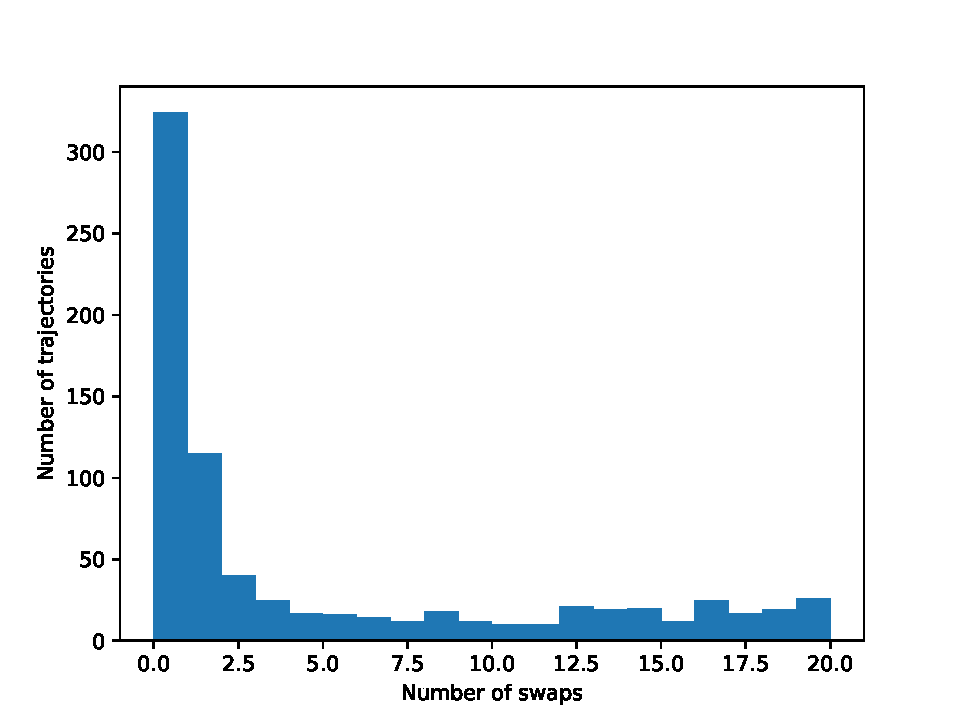
\includegraphics[width=0.45\textwidth]{figures/swaps-distribution-20.pdf}

  \caption{Frequency histograms of number of swaps for trajectories participating in less than 20 swaps.}
  \label{fig:swaps-distribution}%
\end{figure}


\subsection{Privacy measure: Adversary Information Gain}\label{Sec:InfoGain}
 
We define the Adversary Information Gain measure for privacy by adapting the Sensitive Attribute Risk measure from \cite{Salas:2019}. Sensitive Attribute Risk considers the fraction of the published attributes of an individual that is part of its original attributes. 

{\color{blue}
The Adversary Information Gain (AIG) of a user's trajectory is the length of the longest segment without swapping in proportion to the length of the entire trajectory. It is the fraction of the original trajectory that can be disclosed by an adversary who knows that a data point belongs to a user, considering that the adversary propagates the knowledge of such data point to the whole segment in-between swaps. 
}

We plot the distribution function of such measure in Figure \ref{fig:ECDF-max-part-OD} with grid size key as `None' (since we are not conditioning on preserving any ODM here). 
It shows that, for more than 75\% of all
trajectories, the AIG is less than 0.2, for 90\% of the trajectories it is less
than 0.4. For most trajectories, an adversary will thus learn only a
small fraction of the original trajectory. 


\subsection{Privacy when preserving the Origin-Destination Matrix}\label{S:PrivacyODM}
We now consider the effects on the privacy measures of restricting 
swapping to preserve the Origin-Destination Matrix (ODM), introduced in Section~\ref{Sec:SufficientSanitizer}. That is, for two trajectories to
swap they have to share the same starting location or origin and ending location or destination up to some scale (grid size in Fig. \ref{fig:OD}.  
This is in addition to the earlier requirements for allowing a swap ($\tau$, $\chi$).

We define the states or locations used in the ODM by the labelled cells or states in a grid obtained by partitioning the
city into equally sized squares (in units of degrees).  

The start location or origin for a trajectory will be given by the square that its first
measurement belongs to and the end location or destination by the square that its last
measurement belongs to. 
In general, it might be more appropriate to
have start and end locations to be determined by the location of the
trajectory at a certain time of the day. 
However, for keeping it
simple, we choose to use only the first and last measurement.
More generally, our approach allows for an arbitrary set of subsets of the city and arbitrary time-intervals to specify Origins and Destinations in a single ODM, or even a sequence of ODMs, but we use a simple grid-based partition at different spatial resolutions to illustrate the effects on privacy here.  

We empirically evaluate how the preserved privacy changes when we go from having
no grid to having a very coarse grid and then making it finer and
finer.

\begin{figure*}
\centering
  \subfloat[\scriptsize The number of possible swaps depending on the
  grid size.] {
    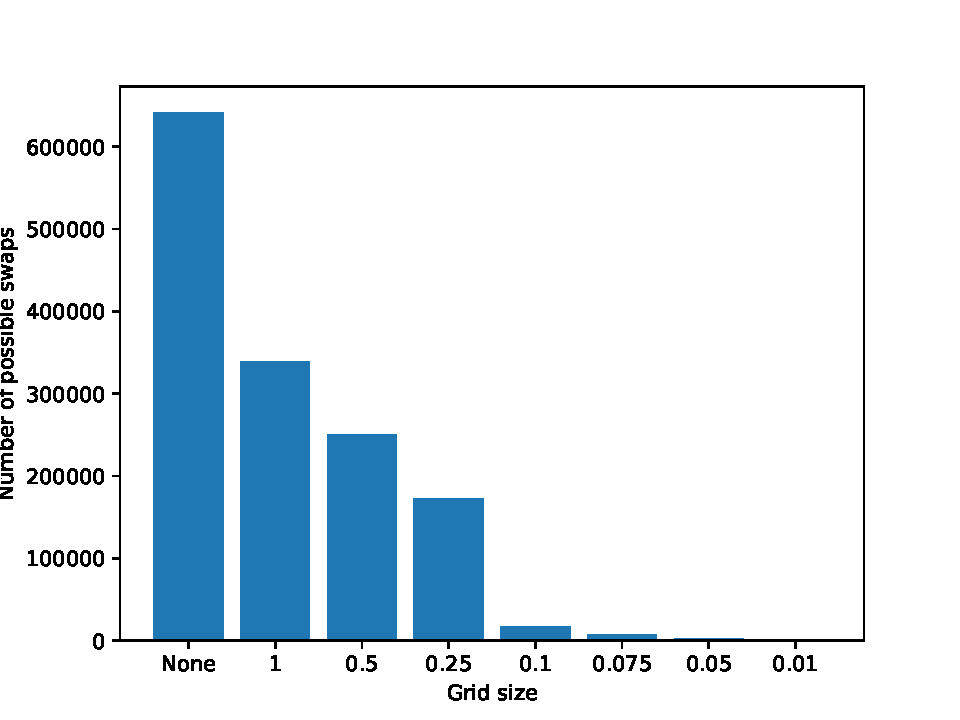
\includegraphics[width=0.45\textwidth]{figures/num-swaps-OD.pdf}
    \label{fig:num-swaps-OD}
  }
%  \hfil
  \subfloat[\scriptsize Empirical Cummulative Distribution Functions of the Adversary Information Gain for different grid
  sizes.] {
    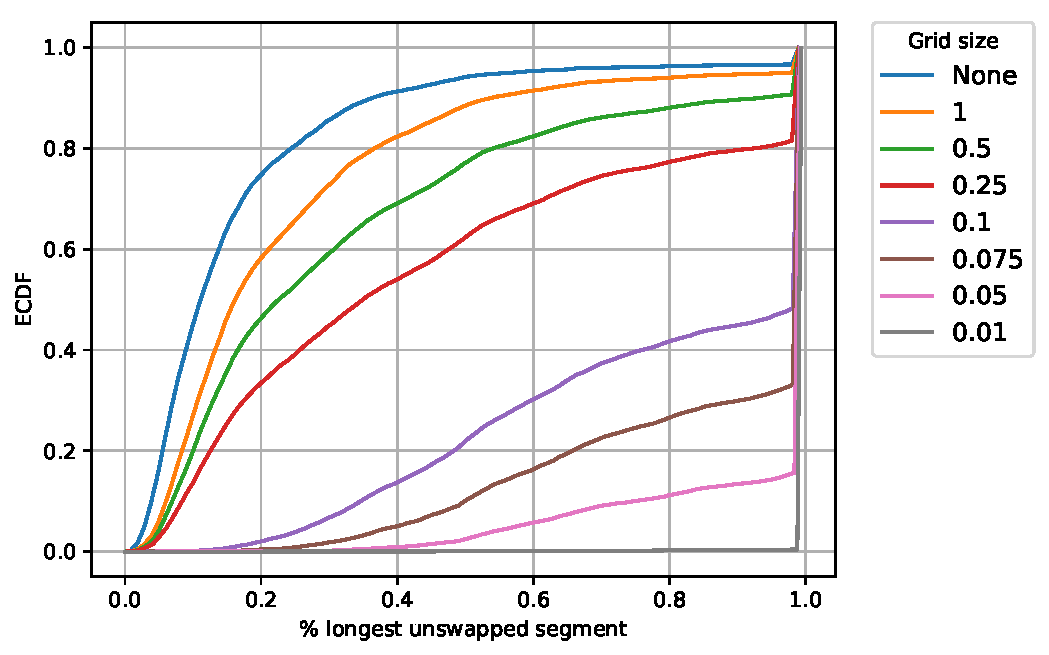
\includegraphics[width=0.45\textwidth]{figures/ECDF-max-part-OD.pdf}
    \label{fig:ECDF-max-part-OD}
  }
  \caption{Preserved privacy when also preserving the ODM}
  \label{fig:OD}
\end{figure*}

In Figure \ref{fig:num-swaps-OD} we see how the number of possible
swaps change when we make the grid finer. At first, we have the number
of swaps without a grid and then we have the numbers for grids of
squares of the given height. The largest height used is 1 degree.
This grid splits the city into four parts, of which two contain
most of the measurements. On the other extreme, the finest grid is made up of squares of width 0.01 degrees which is 10 times the proximity threshold for swappability.  
%We see that the number of possible swaps quickly decreases as the grid
%gets finer. 
{\color{blue} 
Thus, for grid size 1, the sufficient statistics for the trips between the four quadrants NE, NW, SE and SW of Beijing would be preserved, but not to a higher precision as with grid size 0.01. In that case, the sufficient statistics for the trips with same origin and destination up to 1,11 km will be preserved.
}

Since the preserved privacy heavily depends on the number of possible
swaps, we expect it to quickly decrease as the grid becomes finer, see Figure
\ref{fig:ECDF-max-part-OD}. 

%We can conclude that the preserved privacy is greatly influenced by
%the grid size of the ODM. 
If the grid is too fine almost no swaps occur
and the SwapMob algorithm returns almost the original data and preserves no privacy as measured through AIG. 
For very coarse grids the privacy is still reduced but depending on the application it could still
be considered acceptable. 
{\color{blue} This illustrates the trade-off between utility and privacy. If we decrease the grid size, the ODMs are more precise, but at the same time it is less likely that two individuals have the same origin and destination, thus it is less likely that there are possible swaps and therefore the privacy provided decreases.
}

Furthermore, by defining a sequence of ODMs, say $(M_1,M_2,\ldots,M_m)$, specified by arbitrary subsets of space 
and intervals of time $[t_{i,o},t'_{i,o}]$ and $[t_{i,d},t'_{i,d}]$ for each $M_i$, one can increase privacy by increasing the number of swappable trajectories. Such a sequence of ODMs should generally be of greater utility for certain decision problems involving traffic flows. We defer a thorough investigation of sufficient sanitizers that preserve sufficient statistics for such sequences of ODMs across spatial and temporal resolutions in a principled manner for future research.  

\section{Related work}
{\color{blue}
In this section we discuss some of the most relevant solutions for trajectory and location privacy.
}
%\cite{Terrovitis:2008} consider a discrete spatial domain were the user trajectories are expressed as sequences of points of interest (POIs).
%
%
%A similar approach is obtained in \cite{Pensa2008}, transforming sequences by adding, deleting, or substituting some points of the trajectory, while preserving also frequent sequential patterns \citep{Agrawal:1995} obtained by mining the anonymized data.
%

\cite{Hoh2005} and \cite{Hoh06} discuss the use of mobility data for transportation planning and traffic monitoring applications to provide drivers with feedback on road and traffic conditions.
For modelling the threats to privacy in such datasets, they assume that an adversary does not have information about which subset of samples belongs to a single user; 
however by using multi-target tracking algorithms \citep{Reid79analgorithm} subsequent location samples may be linked to an individual who is periodically reporting his anonymized location information.

\cite{Hoh06} consider the attack of deducing home locations of users by using clustering heuristics together with the decrease of speed reported by GPS sensors. Then, propose data suppression techniques by changing the sampling rate (e.g., from 1 to 2, 4 and 10 minutes) for protecting from such inferences.

\cite{Hoh2005} propose an algorithm to prevent adversaries from tracking complete individual paths, it 
perturbs slightly the trajectories of different individuals in such a way that multi-target tracking algorithms are not able to distinguish which segment of the path corresponds to which user.
This is done with a constraint on the Quality of Service, which is expressed as the mean location error between the actual and the observed locations. They argue that adequate levels of privacy can only be obtained if the density of users is sufficiently high.

{\color{blue} Mix Zones, introduced by \cite{Beresford2003}, also prevent applications from tracking complete individual paths. 
%It is closely related to the concept of Mix Zones introduced in \cite{Beresford2003}. These 
They are used to preserve the advantages of location aware services while hiding users' identities from applications that receive their locations.
Applications do not receive traceable user identities, they receive pseudonyms that allow communication between them. Such communication passes through the trusted intermediary and the pseudonyms of users change when they enter a mix zone.
They are spatial areas on which users' location is not accessible, hence when users are simultaneously present on a mix zone, their pseudonyms are changed. This procedure is performed to disrupt the linkage of the incoming and outgoing path segments to the same specific user.
}

To measure the location privacy provided by a mix zone, \cite{Beresford04mixzones} define the anonymity set as the group of people visiting the mix zone during the same time interval. However, as the boundary and time when a user exits a mix zone is strongly correlated to the boundary and time when the user enters it, such information may be exploited by an attacker; therefore they use the information theoretic metric that \cite{Serjantov2002} proposed for anonymous communications. 

This is modeled by \cite{Beresford04mixzones} as a movement matrix that represents the frequency of ingress and egress points to the mix zone at several times.
A bipartite weighted graph is defined in which vertices model ingress and egress pseudonyms and edge-weights
model the probability that two pseudonyms represent the same underlying person. Therefore, a maximal cost perfect matching of these graphs can be used to find the most probable mapping among incoming and outgoing pseudonyms.  
However, since the solution to many restricted matching problems including this one is NP-hard \citep{Tanimoto1978}, \cite{Beresford04mixzones} describe a method for achieving partial solutions.


An approach that does not consider middleware to obtain location privacy is proposed by \citet[Chapter 9]{Gidofalvi2007}. It consists in a system with an untrusted server and clients communicating in a P2P network for privacy preserving trajectory collection.
The aim of their data collection solution is to preserve anonymity in any set of data being stored, transmitted or
collected in the system. This is achieved by means of $k$-anonymization and swapping.
Briefly, the protocol consists in the clients recording their private trajectories, cloaking them among $k$ similar trajectories and exchanging parts of those trajectories with other clients in the P2P network. However, in the final step (the data reporting stage) clients send anonymous partial trajectories to the server; it filters all the synthetic trajectory data generated during the process and recovers the original trajectory.

One of the advantages of performing trajectory anonymization on the user side, as in \cite{Romero-Tris2016} and \cite{Romero-Tris:2018}, is that the anonymization process is no longer centralized. Thus data subjects gain control, transparency and more security for their data.
They leverage the concept of $k$-anonymity for trajectories, similarly to \cite{Abul2008}, that propose the $(k, \delta)$-anonymity model, which consists of publishing a cylindrical volume of radius $\delta$ that contains the trajectory of at least $k$ moving objects. 
Note that this idea is an extension of the concept of $k$-anonymity for databases \citep{Samarati:1998} and it may be related to $k$-anonymity for dynamic databases \citep{Salas:2018-b} if we consider that the records of the dynamic database represent locations.  
Also the concept of differential privacy \citep{Dwork:2006} has been extended from databases to many other types of data.
For a brief overview of privacy protection techniques and a discussion of $k$-anonymity and differential privacy models in different frameworks cf. \cite{Salas:2018}.


\cite{Chen:2012} consider a differential privacy model for transit data publication using data from the Soci\'{e}t\'{e} de Transport de Montr\'{e}al (STM). 
The data are modeled sequentially in a prefix tree that represents all the sequences by grouping those with the same prefix into the same branch.
Their algorithm takes a raw sequential dataset $D$, a privacy budget $\epsilon$, a user specified height of the prefix tree $h$ and a location taxonomy tree $T$, and returns a sanitized dataset $\tilde{\mathcal{D}}$ satisfying $\epsilon$-differential privacy.
For measuring utility, in the STM case, sanitized data are mainly used to perform two
data mining tasks, count query and frequent sequential pattern mining \citep{Agrawal:1995}.


\cite{Xiao:2015} propose a differentially private algorithm for location privacy that follows a discussion on the different notions of adjacency used for  differential privacy \cite{Chatzik:2013,Kifer:2011}.
Their algorithm considers temporal correlations modeled as a Markov chain.
% and proposes the ``$\delta$-location set'' to include all probable locations where the user might appear. 
%The authors argue that, to protect the true location, it is enough to “hide” it in the $\delta$-location set in which any pairs of locations are not distinguishable.
%However, they leave the problem of protecting the entire trace of released locations as future work.

{\color{blue}
There are several other techniques for anonymizing trajectories in data publishing and for 
location privacy, for surveys on these topics, cf. \cite{Fiore:2019} \cite{Primault:2019}.
}  
\section{Conclusions}\label{Sec:conclusions}

We have defined the concept of sufficient sanitizer in which the utility requirement (as a sufficient statistic) is a priori defined, then the sanitization algorithm that preserves such utility is applied to the data.

{\color{blue}
We showed that the SwapMob algorithm is a sufficient sanitizer for counts, transition counts and may be modified to preserve also ODMs.
When applied in real time it may be useful for providing anonymous data to personalized assistants. 


We tested the SwapMob algorithm on the T-drive dataset and defined 
the Adversary Information Gain (AIG) measure to compare the privacy provided when using different grid sizes.
AIG measures the capability of an adversary who knows exact points of the trajectory to infer a larger part of the full trajectory.

We added restrictions to SwapMob to preserve the ODMs and performed experiments to show how AIG
increases when we decrease the grid size for obtaining more precise ODMs.
}
This is the natural tradeoff between the {\em societal utility} gained through the preservation of the ODM, where ODM is a sufficient statistic, and the {\em individual privacy lost} by the sufficient sanitizer.

We remark that preserving sufficient statistics for various statistical decision problems is used in traffic engineering and city planning, including exact count queries, transition count queries and ODM queries, which neither $k$-anonymity nor differential privacy cannot formally guarantee.


A formal privacy-preserving decision-theoretic framework based on probabilistic models and statistical experiments for co-trajectories that can be integrated across multiple spatial and temporal resolutions needs further investigations, especially when the computational setting becomes distributed to handle mobility data at a massive scale.

\section*{Acknowledgements}
Juli\'{a}n Salas acknowledges the support of a UOC postdoctoral fellowship.
This work is partly funded by the Spanish Government through grants  RTI2018-095094-B-C22 ``CONSENT" and TIN2014-57364-C2-2-R ``SMARTGLACIS'', Swedish VR (project VR 2016-03346). Raazesh Sainudiin was partly funded by Combient Competence Centre for Data Engineering Sciences at Uppsala University and the Research Center for Cyber Security at Tel Aviv University established by the State of Israel, the Prime Minister's Office and Tel-Aviv University.



\bibliographystyle{model2-names}

\bibliography{biblio-swap2}

\end{document}
